\chapter{Design and Implementation of Web-based IoT Applications}
\label{chapter:Design-and-Implementation-of-Web-based-IoT-Applications}

\section{Patterns for Web-based IoT Applications}
\label{chapter:Patternsforweb-basedIoTapplications}

\subsection{RPC}
Remote Procedure Call (RPC) is one of the Inter-Process Communication methods for data exchange among threads or processes on different hosts. Unlike a local application case \cite{srinivasan1995rpc}, where the code runs all locally, RPC solves the problem of excusing codes of the whole application which is distributed cross different networks or the Internet.

RPC can be further developed into a massage pattern\footnote{http://wamp.ws/faq\#rpc} involving two roles, client and server. Usually, RPC pattern is initiated by a client, which sends an request to a remote server; The server processes based on the request, then responses to the client. An example of RPC pattern is shown in Figure \ref{fig:RPC-pattern}. The client starts its procedure sequence when the programme is running. The procedure sequence starts with Procedure 1. The client, afterwards, needs the result from Procedure 2 which locates on the Server. Thus, it sends a request to the server. The server handles the logic when the request comes, and thus it starts Procedure 2. At the moment, the Client is waiting for the result until the server responses to the client. With the result, the client can now continue to execute the next procedure, Procedure 3.  

\begin{figure}[ht]
  \begin{center}
    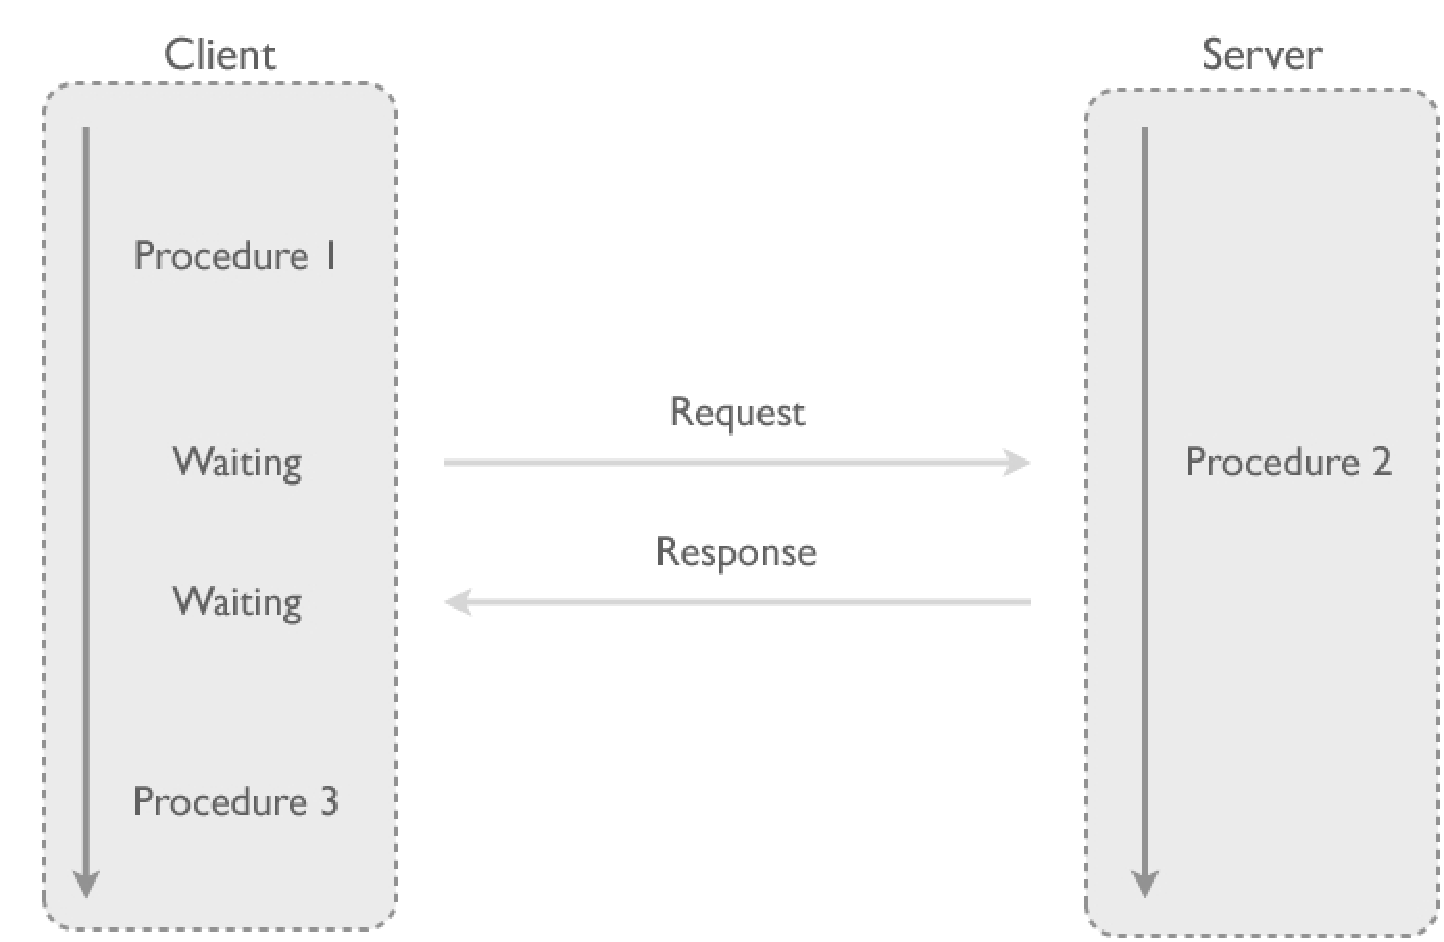
\includegraphics[width=1\textwidth]{images/RPC-pattern.pdf}
    \caption{An Example of RPC Pattern}
    \label{fig:RPC-pattern}
  \end{center}
\end{figure}

RPC is commonly used in real world scenarios. For example, Facebook, a social network web platform, provides open APIs that allows third party applications to access its data. Here, Facebook plays the role of the server(s), while the third party applications play the role of the client. When a third party application (client) sends a request to Facebook asking, e.g. a list of the user's friends, Facebook servers process the request. Facebook servers, then, response to the client, when the result, either success or error, is ready. The client can then use the list of friends to perform further procedures. 

From the perspective of IoT, RPC pattern covers one of the two most important interaction in the IoT application architecture, i.e., sending commands or configuration control. In the case of IoT, nodes could locate on different locations from cities to countrysides. Commanding is helpful to configure a node remotely, e.g. setting the parameters (device identification, timeout and reporting rate). As for an actuator, RPC pattern can control its action. e.g. a light actuator, or called a light switch, has the actions of on and off. With commanding, the light can, thus, be switched on or off remotely.

\subsection{Publish/Subscribe}

Publish/Subscribe (Pub/Sub) is one of the messages exchange patterns. Messages are exchanged based on publishing and subscribing. A sender of a message is called a publisher. Usually, each message contains a topic. A receiver filters and receives a message by the message topic. The receiver who subscribes topics is called a subscriber. 

Pub/Sub architecture consists, usually, at least publishers, subscribers and a broker(s). The broker maps the right messages to the right receivers and exchanges messages among publishers and subscribers. Generally, there is, on one hand, no restricted boundary between a publisher and a subscriber. This means, a publisher can also be a subscriber and receives messages from other publishers; while a subscriber can also be a publisher and publishes messages with topics. On the other hand, there is no order between publishing and subscribing. This means, a publisher can publish a message with a topic without subscribing any topic; or even no one subscribes the topic. The subscriber does not have to subscribe any topic either. This refers to, if the aforementioned situation happens, then messages are , e.g., simply discarded. All the message exchanging logics, however, are handled by the broker(s). The broker(s) should specifies and implements corresponding functions to different messaging situations. 

An example of Pub/Sub pattern is shown in Figure \ref{fig:publish-subscribe-pattern}. Client 1 plays roles in both subscriber and publisher in different stages. i.e., When it subscribes topic 1, client 1 is treated as a subscriber. Client 1, however, changes to a publisher when it publishes a message with the topic (topic 1). The broker analyses the message and maps the topic to the subscribers who are interested in the topics. In this case, both Client 1 and Client 2 are interested in the topic. Hence, the broker replies the message to both of them. Client 1, and thus, changes its role to a subscriber.

\begin{figure}[ht]
  \begin{center}
    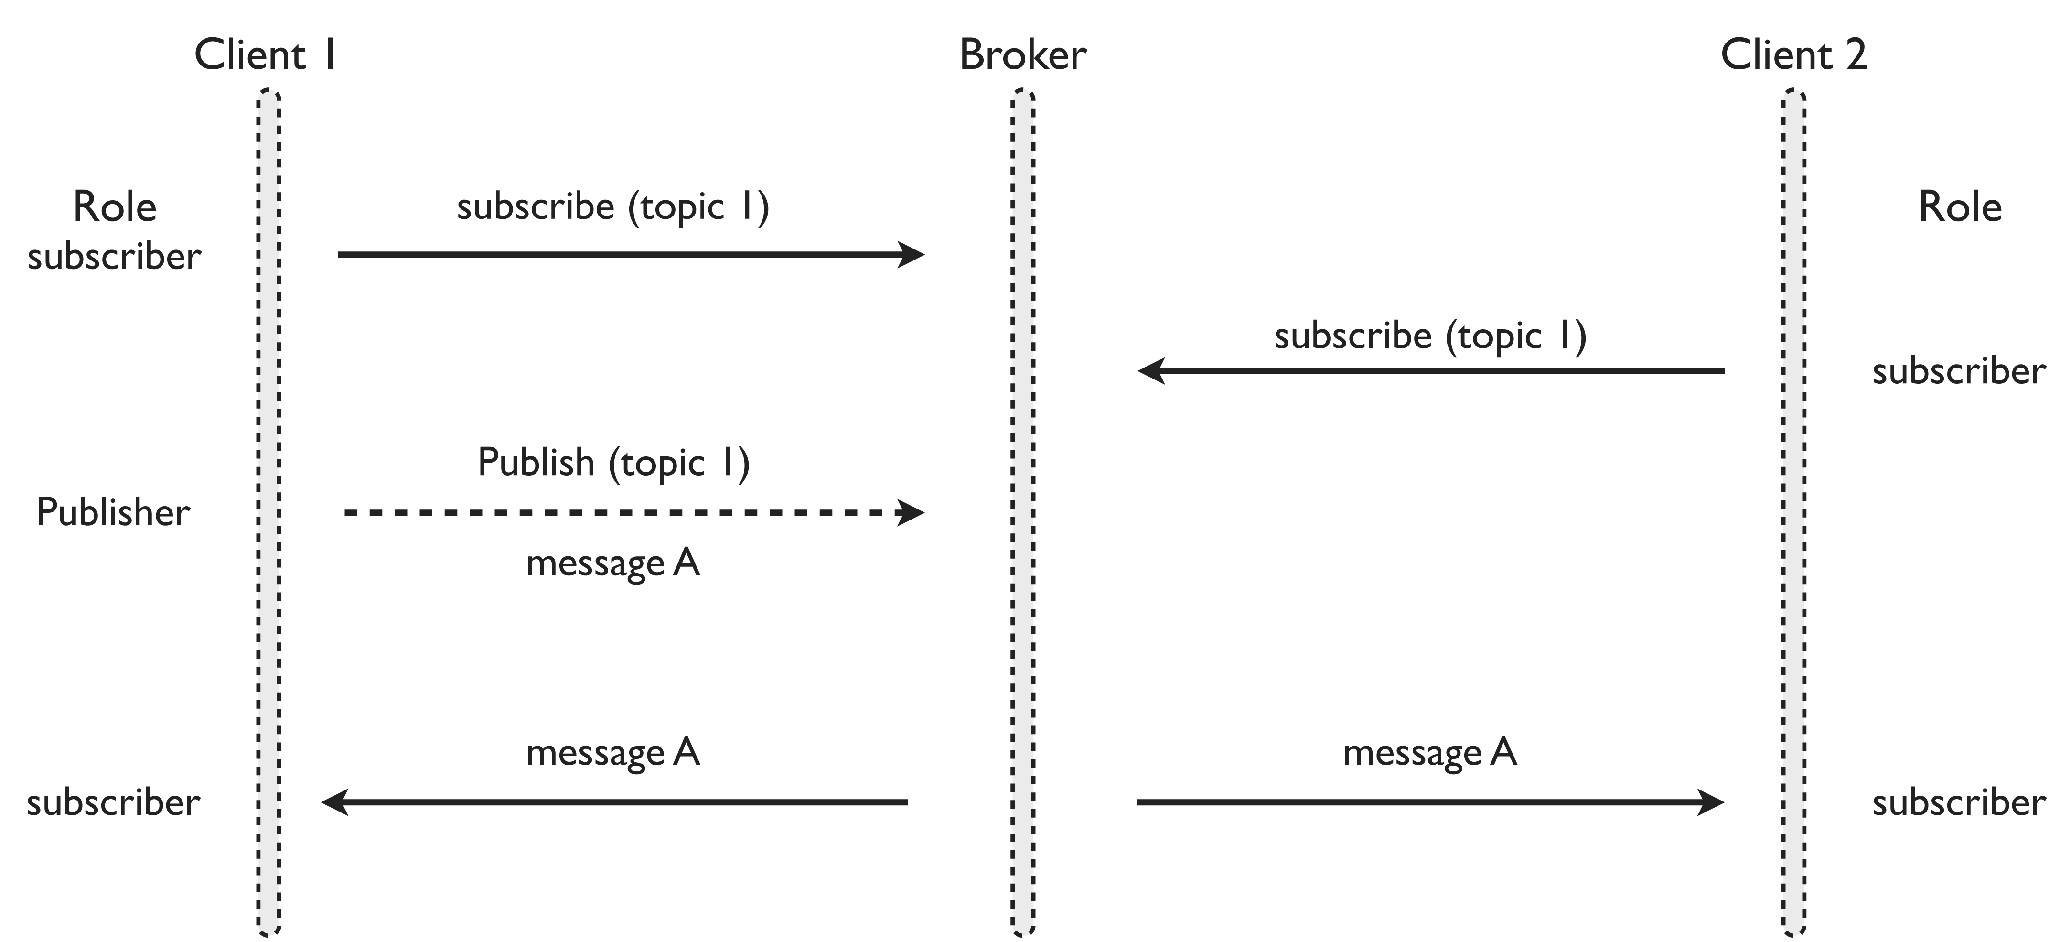
\includegraphics[width=1\textwidth]{images/publish-subscribe-pattern.pdf}
    \caption{An Example of Publish/Subscribe Pattern}
    \label{fig:publish-subscribe-pattern}
  \end{center}
\end{figure}

The concept of Pub/Sub pattern has been used in real world cases. Twitter, for example, can be treated as a real world scenario, even though the implementation might be different in Twitter. When a new user, User 1, posts a message in Twitter, usually, it will not popup on any other users' home page, but it will popup on User 1's homepage or a similar page that represents the user. This can be understood that User 1 subscribes himself, but no one subscribes him. 

User 1 can follow other users based on his interest. For example, User 1 follows User 2. User 1 will, then, receives User 2's post on User 1's homepage. Here, User 2 becomes a topic that User 1 subscribes; User 1 is the subscriber and User 2 is the publisher. Twitter, acts as a broker, handles the logic how the messages sent by User 2 delivers to User 1.

From the perspective of IoT, Pub/Sub pattern covers the other one of the two most important interaction in the IoT application architecture, i.e., notification. With notification, data can be sent interconnected, such as among nodes or from nodes to data centres. For example, one node, Node A, collects temperature data and humidity data. Node A then submits the collected data to the other node or data centre (called Node B) for the purpose of assembling. One strategy, which organises and manages the data sent by Node A, is to set the topic of the each message to the data type (i.e., temperature or humidity). Subsequently, Node B can easily categorise the data for further processing.

\subsection{Database-centric Approach}
Database-centric is a software architecture where database plays critical role. Generally, database provides fault tolerant and reliable transactions. Database-centric Approach, in IoT services, subsequently, provides a dependable mechanism to record enormous IoT data. 

An example of implementing a database-centric IoT service has been discussed in \cite{francesco2012storage}. The approach merges the features of database-centric approach with the demands of IoT services, and provides customised features for IoT services. Thus, the approach, firstly, supports heterogeneous and multimedia contents; Secondly, it provides standard APIs for standard web services, and thus the IoT data can be utilised at optimally maximum; Finally, live notification is supported and security features are applied.

\section{Smart Lighting and Control Application}
\subsection{Components}
In the thesis, we built an HTML5 based application to demonstrate a smart lighting and controlling IoT service. The concept of the sample service consists the following elements: a light, a switch, a sensor and the sun. The light is a component that visualises the light status. The switch is a component that represents an actuator that can control the light. The sensor is a component that senses the environment brightness. The sun represents the environment. The change of the luminance from the sun affects on the sensor which then affects on the light. The luminance of the light will be, subsequently, adjusted. The service allows the light to keep the brightness of a space constantly, or to be adjusted by the switch: on, off or to dim. The relationship among the components is shown in Figure \ref{fig:components-relationship}. 

\begin{figure}[ht]
  \begin{center}
    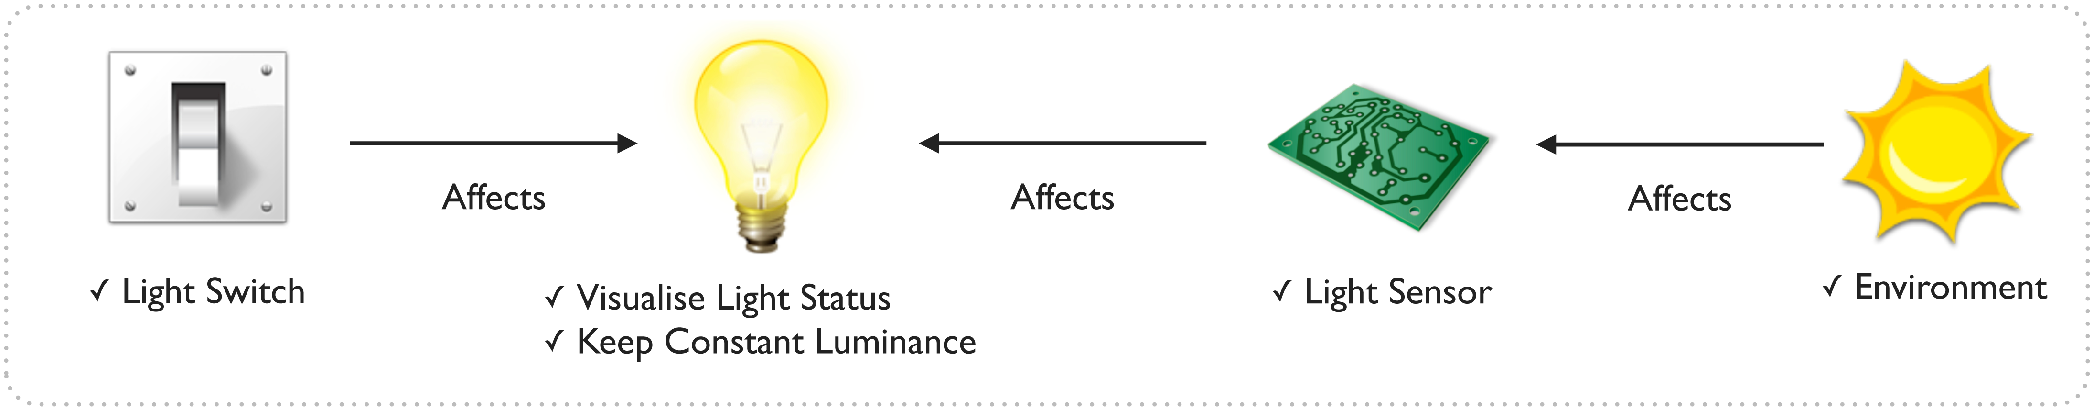
\includegraphics[width=1\textwidth]{images/components-relationship.pdf}
    \caption{Components of The Smart Lighting and Control Application and Their Relationship}
    \label{fig:components-relationship}
  \end{center}
\end{figure}

\subsection{Implementation of The Backend}
With the concept above, we implemented an embedded web server based on a NodeJS. We also attached a WebSocket server to the NodeJS, and a WAMP server on top of the WebSocket server. The embedded web server, then, understands the WebSocket protocol and the WAMP subprotocol. The component layer structure is shown in Figure  \ref{fig:component-layer-structure}. 

\begin{figure}[ht]
  \begin{center}
    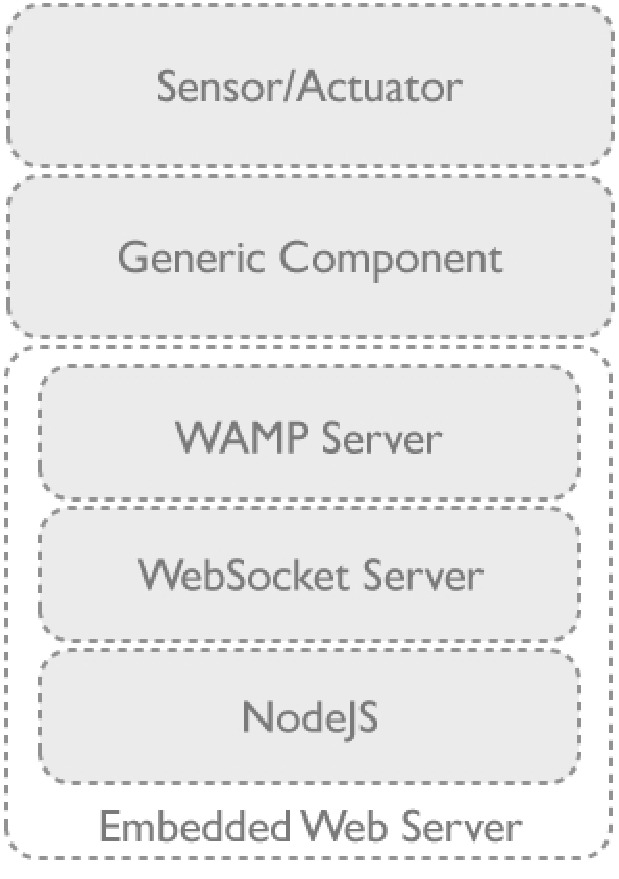
\includegraphics[width=0.5\textwidth]{images/component-layer-structure.pdf}
    \caption{Component Layer Structure}
    \label{fig:component-layer-structure}
  \end{center}
\end{figure}

We added a generic component layer on the embedded web server. The generic component is an abstract layer that describes information and generic configuration of a device, e.g., component type (temperature sensor, humidity sensor or light actuator etc), device ID, returnable, timeout, data sent rate and some other hardware parameters. 

The generic component also implements a function that control the component events. For example, if the sensor should send the data in some fixed interval or the data should be sent only by signalled. In the thesis, the generic component covers sensor and actuator. Thus, we added another component layer onto the generic component. All the layers interconnected will, subsequently, play the role of sensor or actuator.

We start with the sensor. As a sensor is built on top of a generic component which handles parameters configuration and event abstraction, a sensor is capable of responding to configuration and events. As for a light sensor, the events are the followings:

\begin{itemize}
% You can use this command to set the items in the list closer to each other
% (ITEM SEParation, the vertical space between the list items) 
\setlength{\itemsep}{0pt}
\item \emph{Get current sensor data}. This function triggers a sensor to retrieve data from its environment. In the sample, the sensor senses light brightness data.
\item \emph{Configuration}. To configure a sensor with parameter. Sensor's action, however, is usually hardcoded and cannot be configured remotely. This is due to a security reason, that the currently implementation does not allow an action parameter (such as a function) transmitted remotely.
\item \emph{Reset}. To reset the configuration of a sensor to default.
\end{itemize}

As for actuator, it is built at the same layer as that for sensor, and thus, it also inheres features from generic sensors as the sensor does. In the sample, we configure an actuator into a light switch, and it can be described as the followings:

\begin{itemize}
% You can use this command to set the items in the list closer to each other
% (ITEM SEParation, the vertical space between the list items) 
\setlength{\itemsep}{0pt}
\item \emph{Switch on}. To switch on a light and regardless the light current state.
\item \emph{Switch off}. To switch off a light and regardless the light current state.
\item \emph{Switch a light}. To switch the light to its opposite state. This means, if a light is on, it, then, will be switched off and vice versa.
\item \emph{Adjust luminance}. To adjust a light luminance to a given value which should be in the range of a light acceptable value.
\item \emph{Configuration}. Similar to that of a sensor.
\item \emph{Reset}. Similar to that of a sensor.
\end{itemize}

In effect with simulation, we added an virtual component that simulates a light. Thus, a light status (on or off) can be check through this component. 

Summary so far, the interface of a light sensor/switch (sensor/actuator) can be illustrated in Figure \ref{fig:component-interface}. in a generic way.

\begin{figure}[ht]
  \begin{center}
    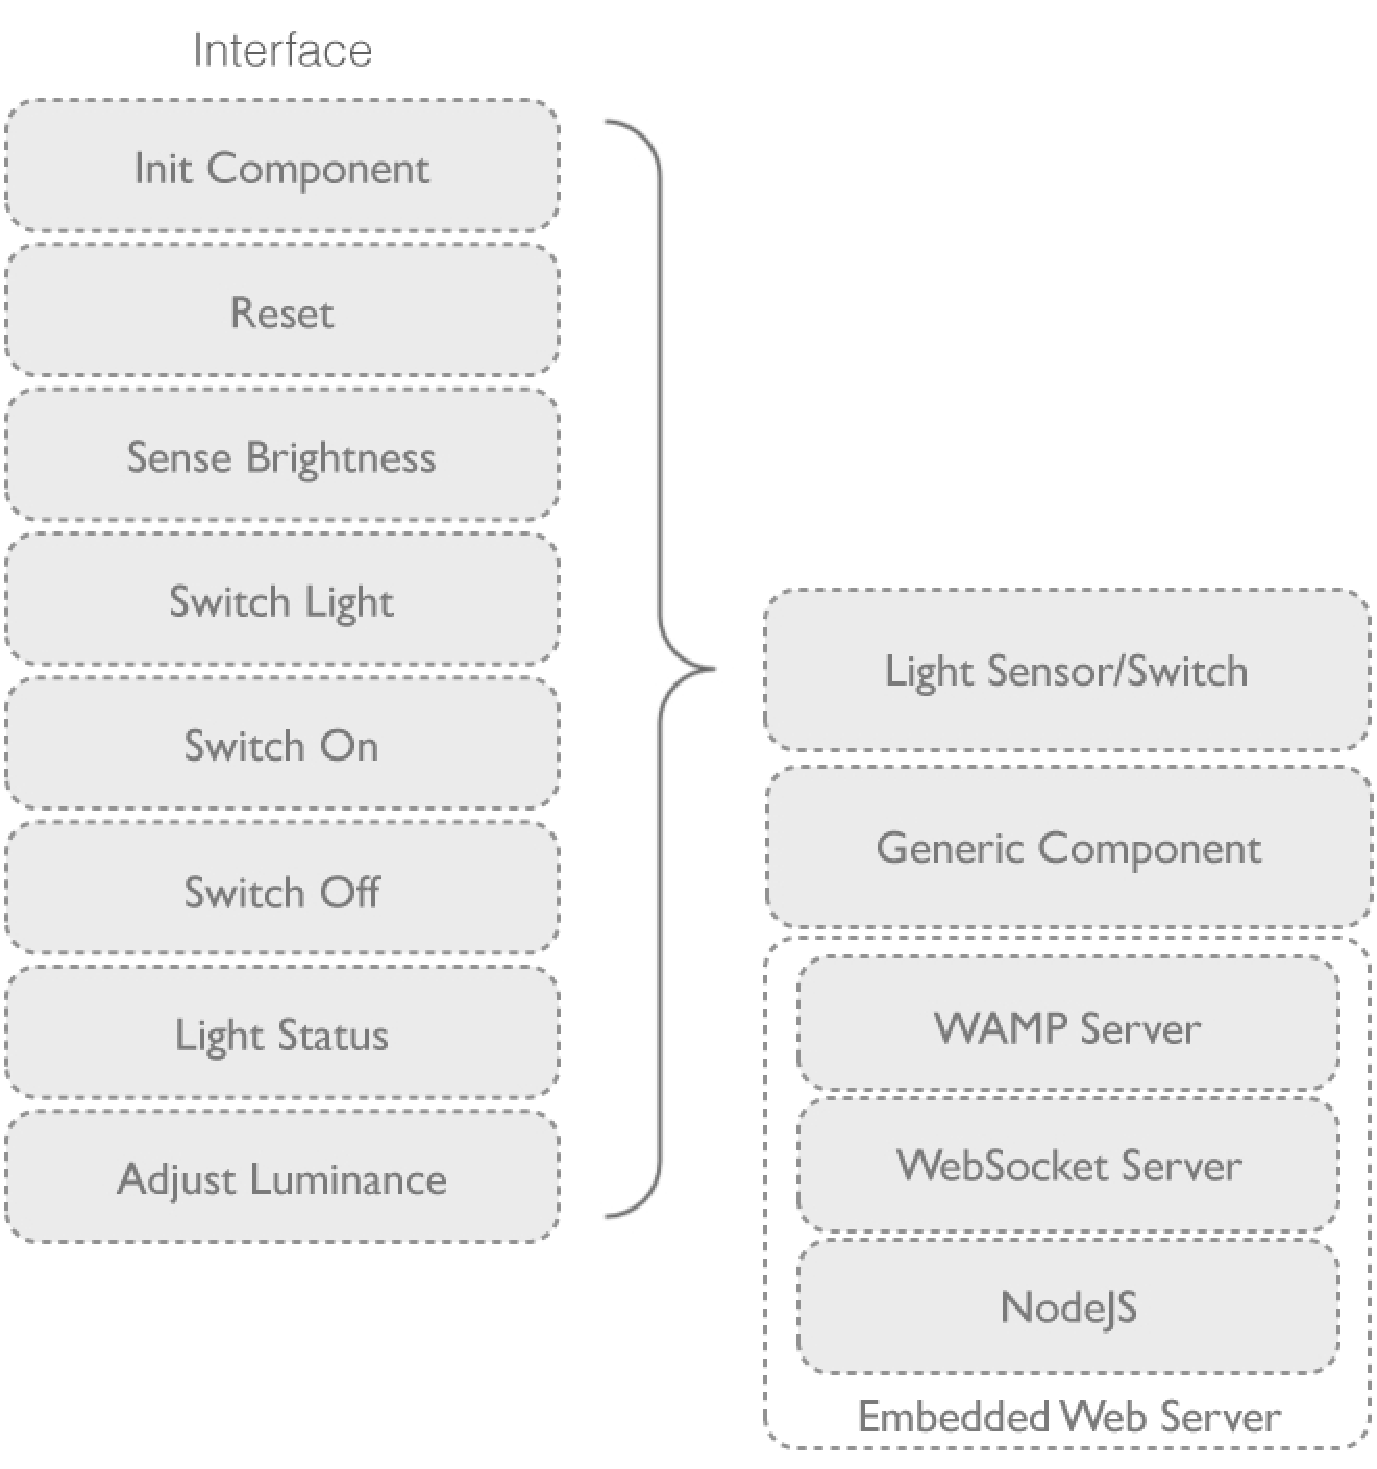
\includegraphics[width=0.7\textwidth]{images/component-interface.pdf}
    \caption{Component Interface}
    \label{fig:component-interface}
  \end{center}
\end{figure}

To view the architecture, at a higher level, which we have exposed so far, the light sensor and the light switch are connected to a component with an embedded web server, or separately. This architecture is shown in Figure \ref{fig:component-nodeJS-interface}.

\begin{figure}[ht]
  \begin{center}
    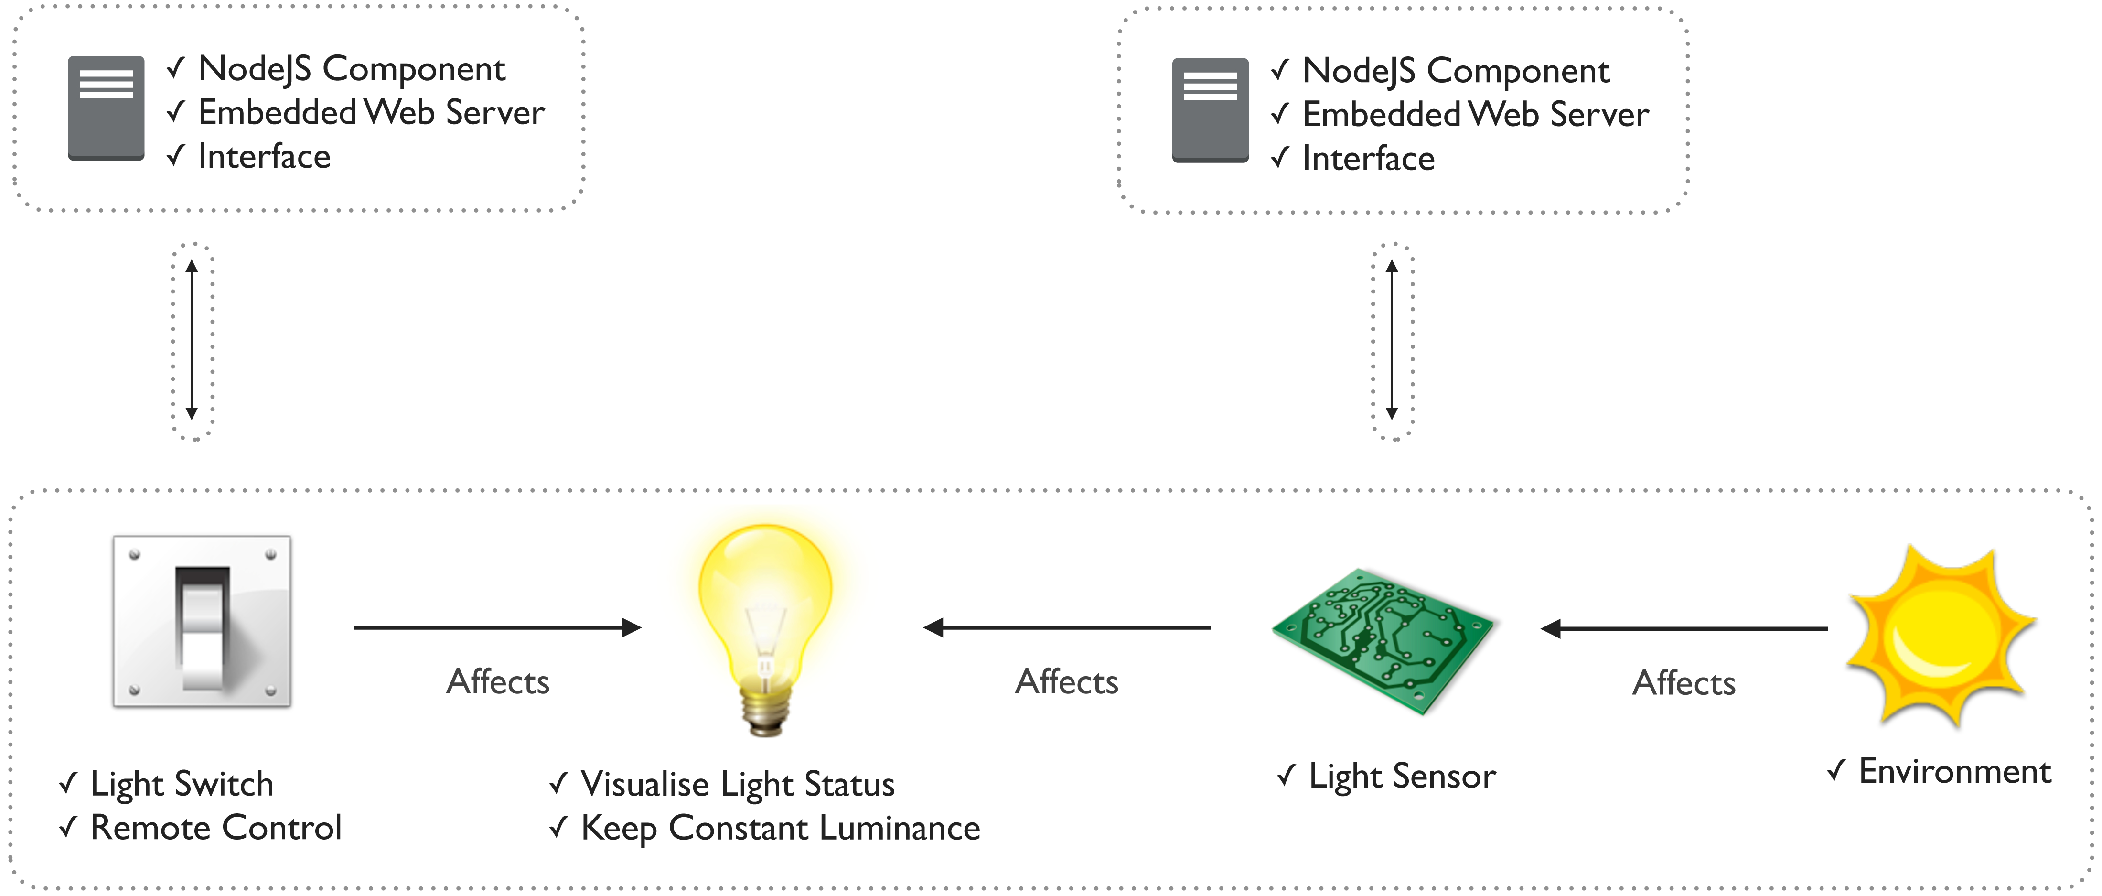
\includegraphics[width=1\textwidth]{images/component-nodeJS-interface.pdf}
    \caption{Components Connected to the Embedded Web Server}
    \label{fig:component-nodeJS-interface}
  \end{center}
\end{figure}

The light sensor and the light switch are linked to a component respectively. The two components differ themselves by the topmost layer which we showed in Figure \ref{fig:component-layer-structure}. With the embedded web server, the light sensor and the light switch can communicate with each other and other components (such as the simulated component, light) over WebSockets. We can think this way, the component, which the light switch connected to, enhance the functionality that the light switch can do. For example, it controls the light via the interface switch on/off. 

\subsection{Implementation of The Front-end}
However, the current system should be accessible from outside, such as by end users. We implemented this via a web front-end interface. 

The structure is layered at front. Concerning the connection is over WebSocket, a WebSocket layer is arranged at the bottom. The WebSocket layer handles the connection with the embedded web server. 

The communication coming from the embedded web server, is however, using WAMP protocol. Thus, we added another layer, WAMP layer, on top of the WebSocket layer. With these two layers, the front-end and the backend can, now, communicate.

We also would like to control the backend, and thus we added another layer, APIs layer, on top of the WAMP layer. The APIs layer contains light sensor APIs and light switch APIs. As the name implies, programmers can control the backend through the APIs that this layer provides. For example, with the APIs, we can make a web interface that visualises the light switch which can response to users click event and subsequently control the light on and off; we can also visualise the light status on a web interface, so we can check the light status remotely. 

This architecture is shown in Figure \ref{fig:front-end-layer-structure}.

\begin{figure}[ht]
  \begin{center}
    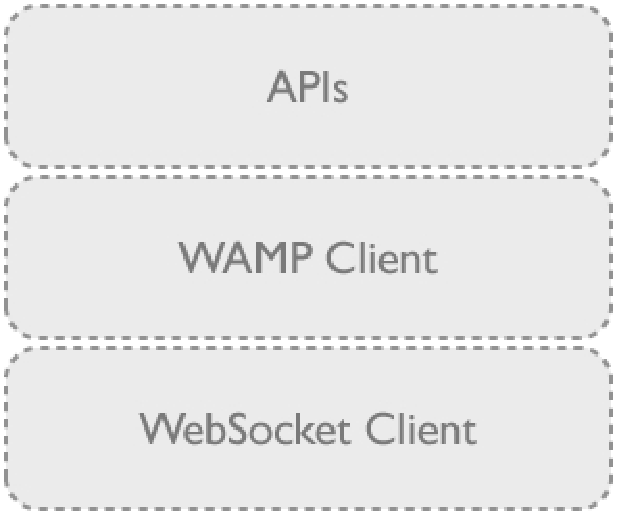
\includegraphics[width=0.5\textwidth]{images/front-end-layer-structure.pdf}
    \caption{Front-end Layer Structure}
    \label{fig:front-end-layer-structure}
  \end{center}
\end{figure}

\subsection{Overall Structure}
We have covered end users, front-end structure and backend structure. Now, we can link them together. This architecture is shown in Figure \ref{fig:communication-structure-with-user}.

\begin{figure}[ht]
  \begin{center}
    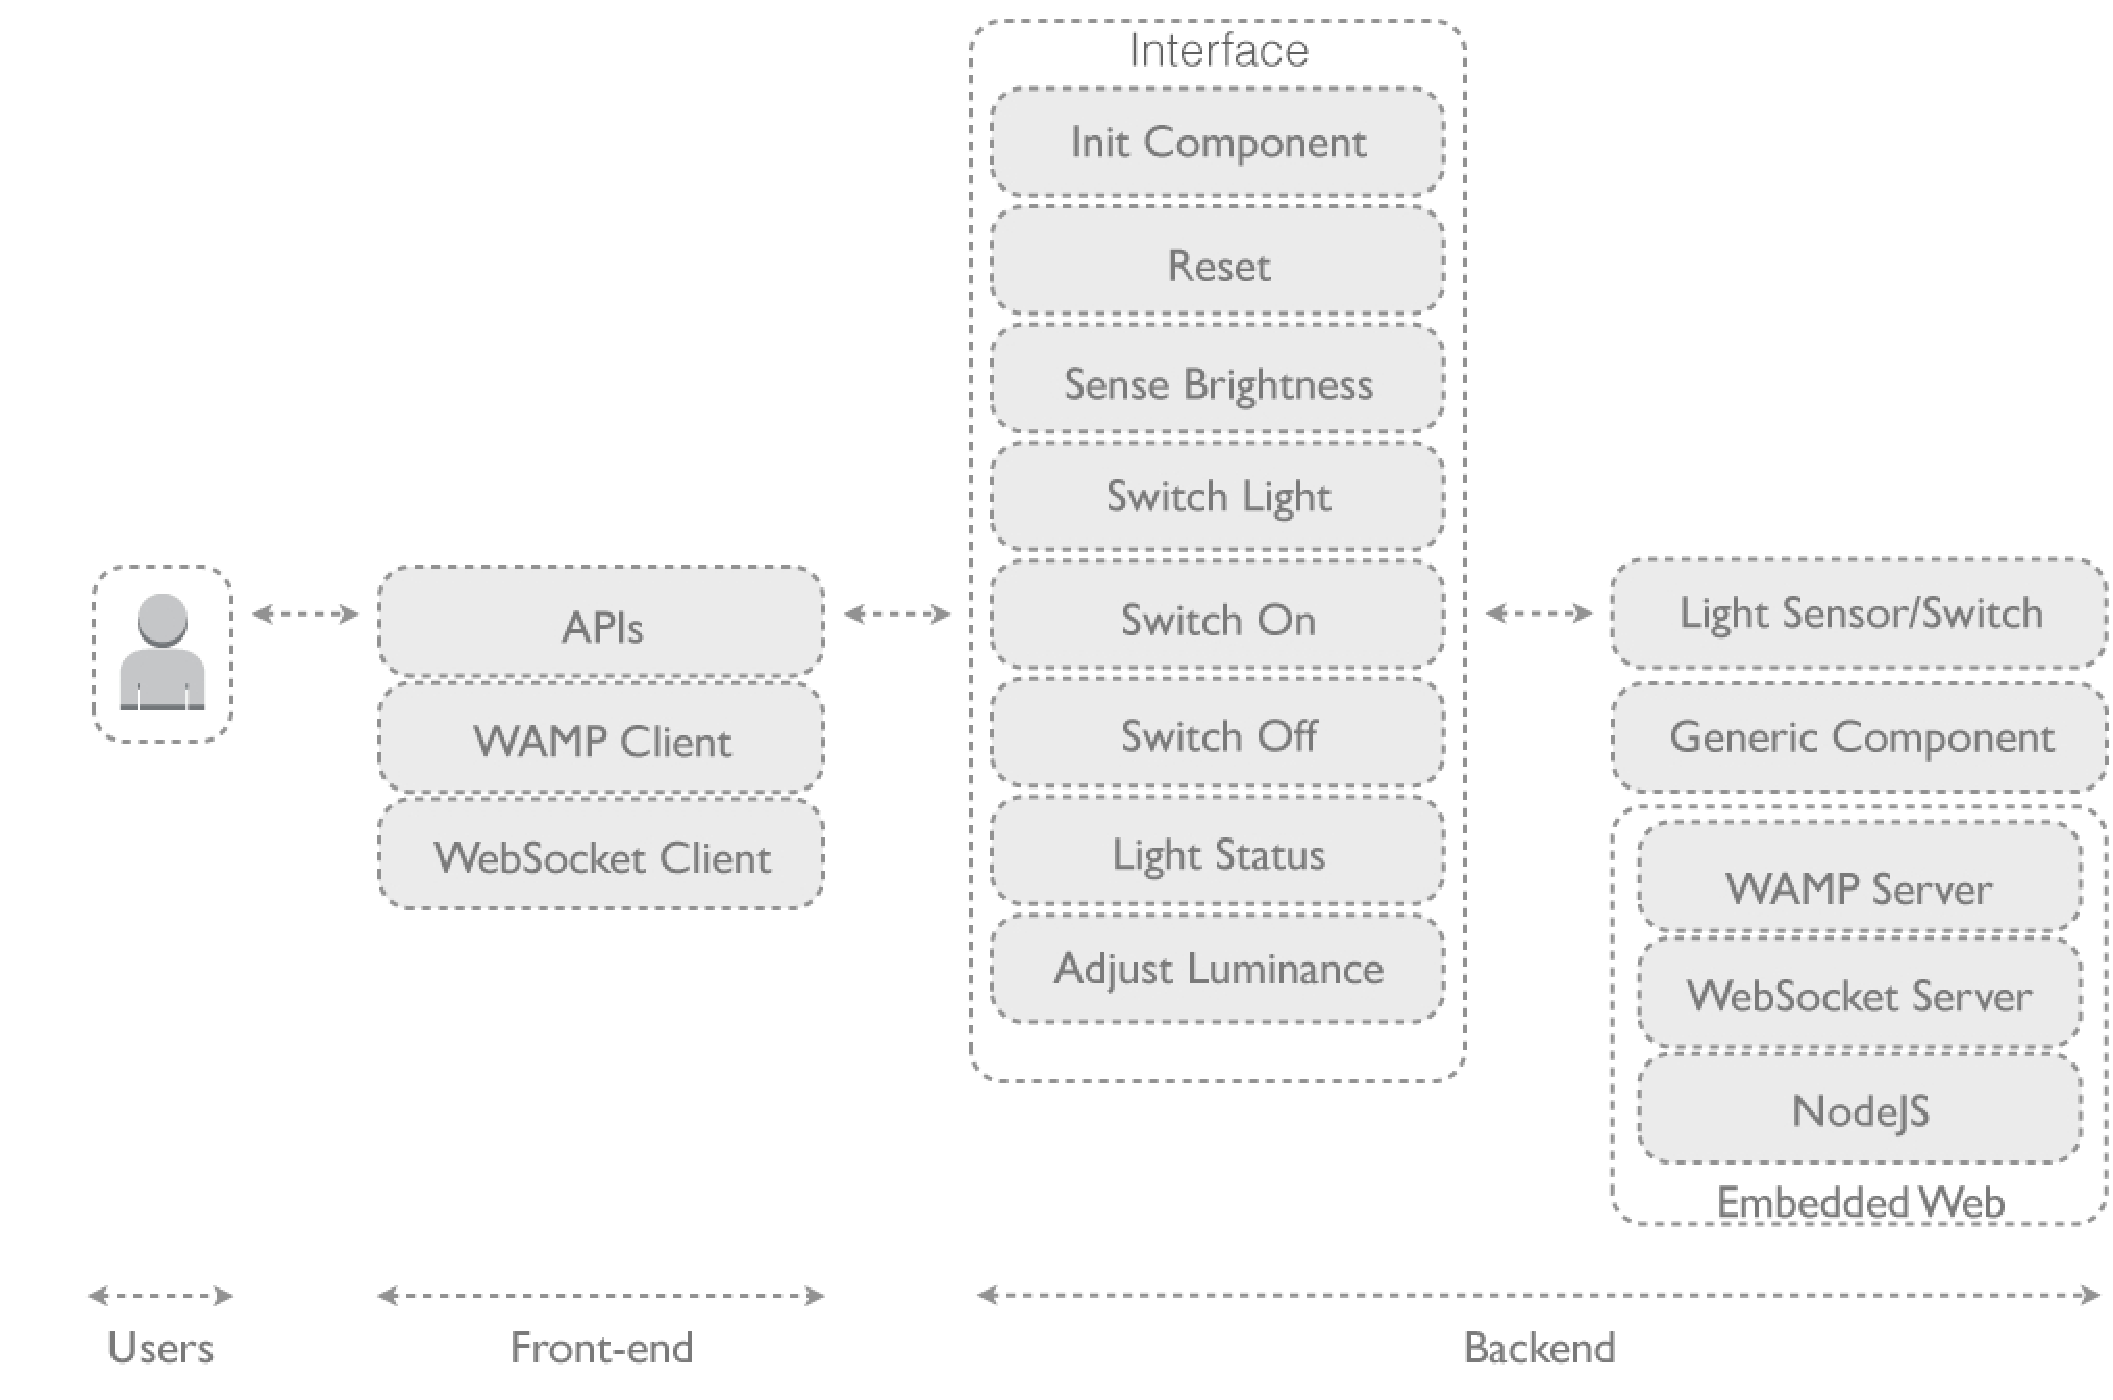
\includegraphics[width=1\textwidth]{images/communication-structure-with-user.pdf}
    \caption{Overall Structure}
    \label{fig:communication-structure-with-user}
  \end{center}
\end{figure}

The APIs layer connects users and the interface provided by the backend. WAMP Client talks with WAMP server through WebSocket Client which talks with WebSocket Server.

\subsection{The Role of Messaging Patterns}
Previously, we have discussed Pub/Sub and RFC. These two pattens, handled by WAMP layer, cover the two most important interactions in Internet of Things: notification and command. Here, we discuss how are they integrated in the sample. This architecture with message patterns is shown in Figure \ref{fig:message-pattern-overall-structure}.

\begin{figure}[ht]
  \begin{center}
    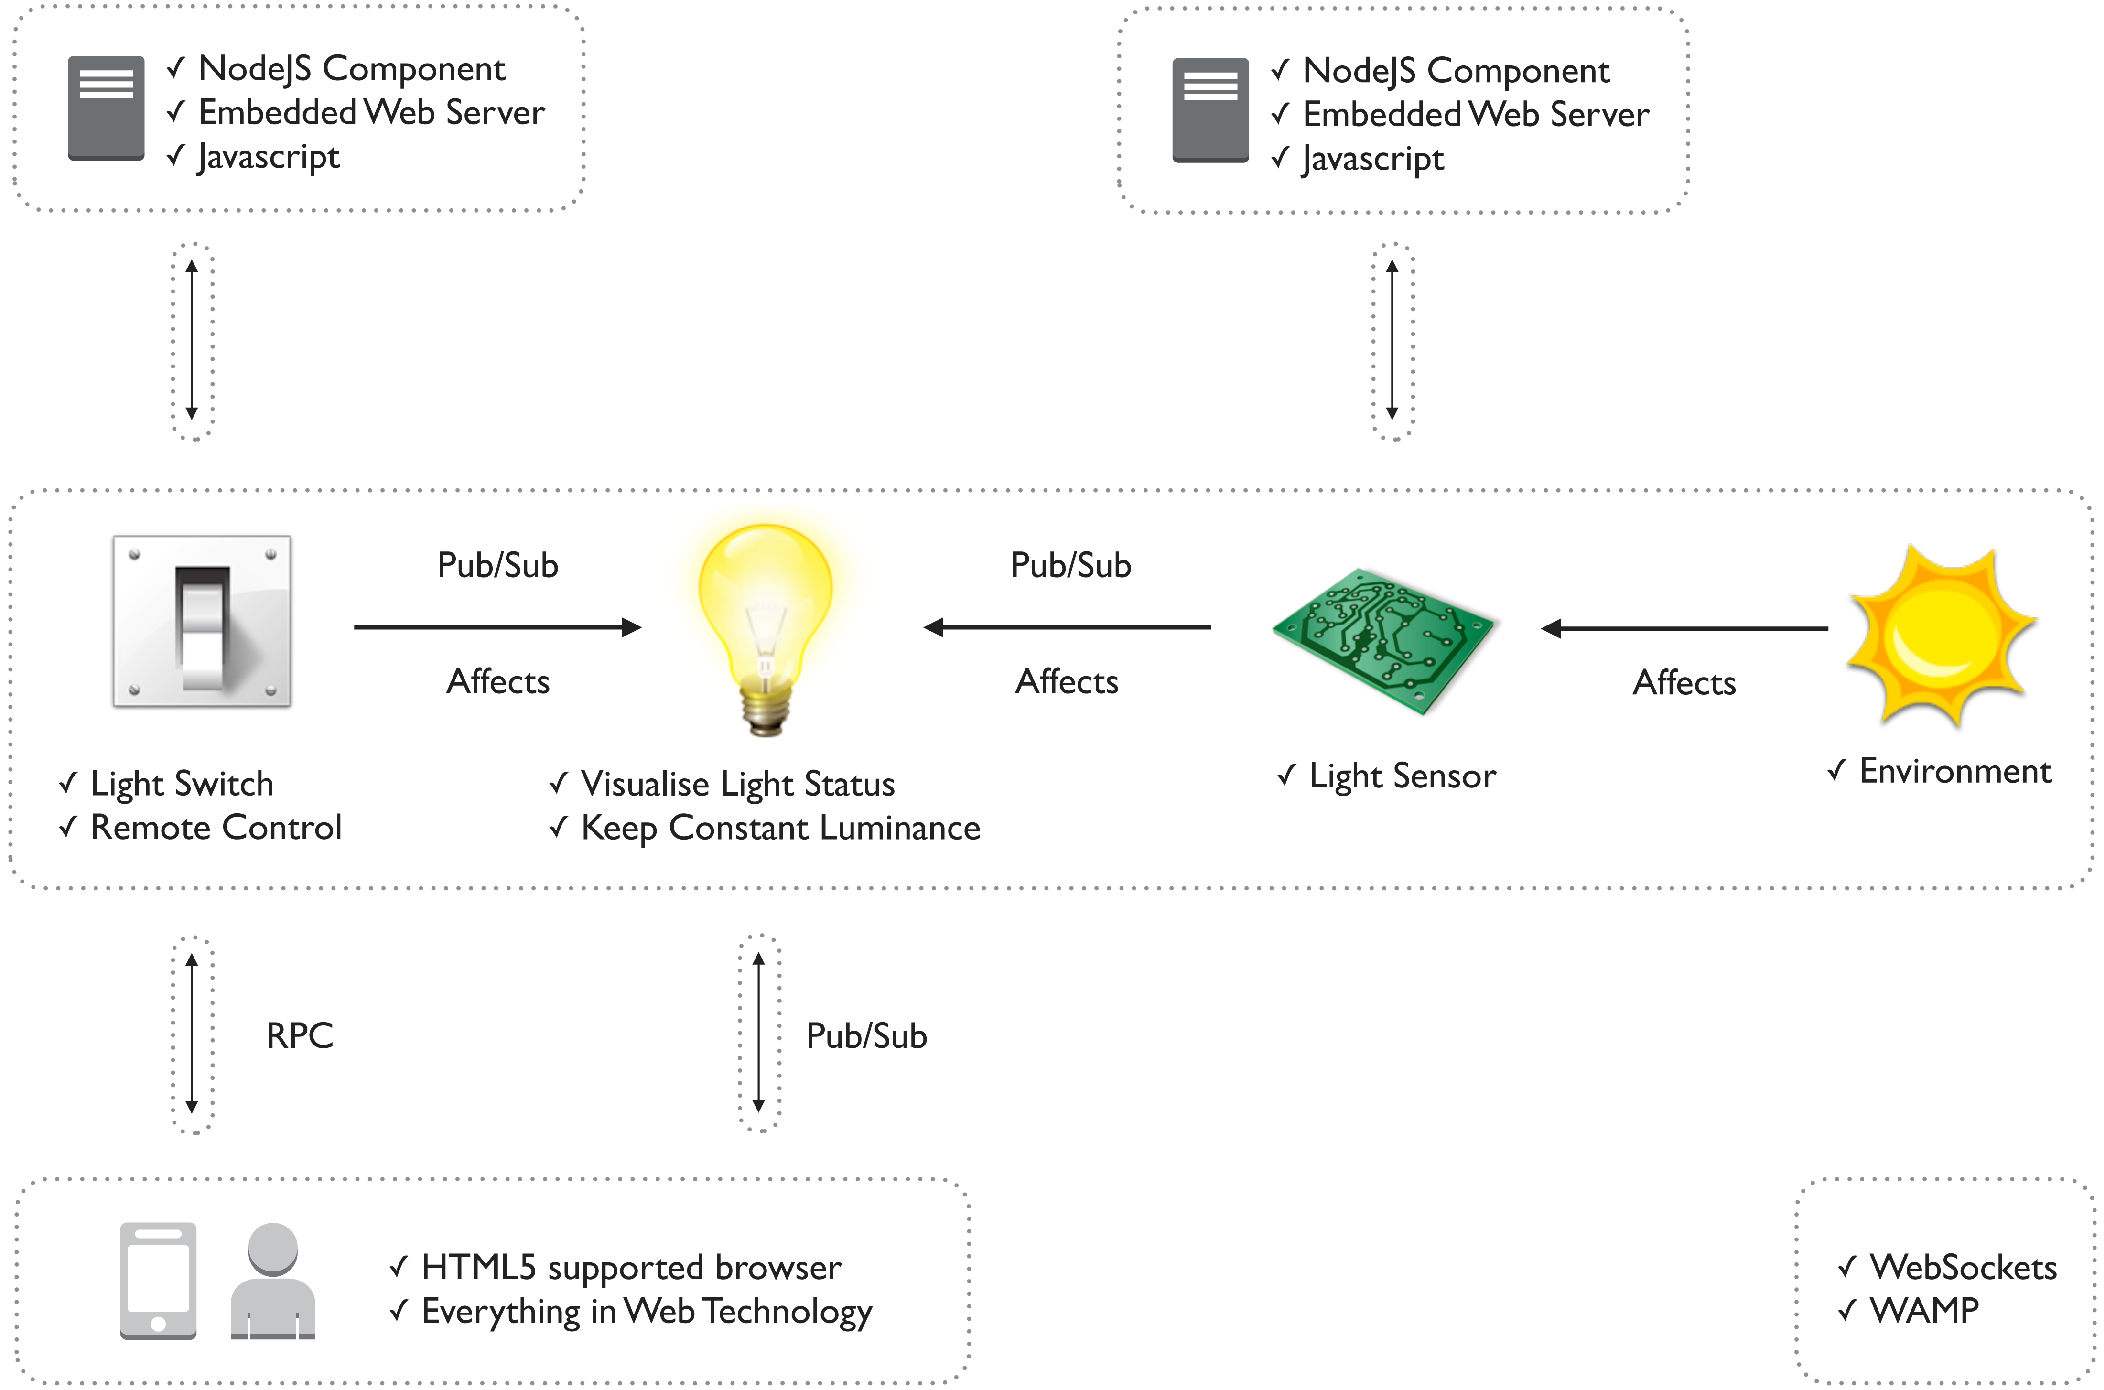
\includegraphics[width=1\textwidth]{images/message-pattern-overall-structure.pdf}
    \caption{Overall Structure with Massage Patterns}
    \label{fig:message-pattern-overall-structure}
  \end{center}
\end{figure}

As the front-end is built with HTML5 technology, the sample is capable with any browser that supports HTML 5 feature (WebSocket). Thus, the architecture is designed in a way that end users can control the light switch and view the light status via a browser. 

When a end user control the light switch, such as turning on the light; turning off the light; or adjusting the luminance of the light, it sends the command using RPC patterns. RPC pattern is also applied in component initialisation and reset. When the user view the visualisation of the light status, it communicates with the components via Pub/Sub patterns.

The interaction between the light switch and the light is using Pub/Sub pattern. The light component subscribes a topic from the light switch. When the user e.g. turns on the light, the switch component publishes a message with the light on value (such as, true) to the light component. The light component, then, receives the message, processes the message and turn on the light. Luminance adjustment is similar.

The interaction between the light sensor and the light is, also, Pub/Sub pattern. The light component subscribes a topic from the light sensor, as opposed to that from the light switch. When the light sensor updates its collected data, the light receives the data and subsequently adjust the light luminance according to its setting.

\section{Social Sensing}
In contrast to the WebSocket based sample: Smart Lighting and Control Application, we provided another sample IoT service, Social Network IoT Sensing Application, based on data centralised model using HTTP for communication. 

\subsection{Features}
The sample application provides a way to visualise data collected by IoT devices remotely in nearly real-time. For example, a user deploys IoT devices at home. The devices, then, collect temperature, humidity and multimedia (image, video, and audio) data at home. The purpose of the design enables the user to inspect those data in a visualised way from a browser. Visualisation means, for example, a graph chart of the temperature of the user's home within the past 24 hours. Real time means, for example, the web interface updates corresponding to live notification, once the collected data have been processed.

Furthermore, the sample application is extensible by integrating third party APIs. For example, the sample could visualised IoT devices geo-locations and geographic structures, with Google Map APIs; Notification could be extended into the area of social network, other than the owner exclusively. 

The underlying infrastructure of application handles scaling such as distributing and clustering. This feature satisfies the same demand in IoT services.

\subsection{Stack and Architecture}
Social Network IoT Sensing Application is a CouchApp\footnote{http://couchapp.org/page/index}, a Javascript and HTML5 application served directly from CouchDB. CouchDB is a documented-oriented database. Data are stored in JSON documents and are accessed with a web browser via HTTP. CouchDB is, also, designed for data distribution and replication. In short, CouchDB provides scalability and flexibility. These features are meaningful to the challenges\cite{francesco2012storage} - heterogeneity and scale - in IoT services. Its layer stack is shown in Figure \ref{fig:data-centre-app-stack}.

\begin{figure}[ht]
  \begin{center}
    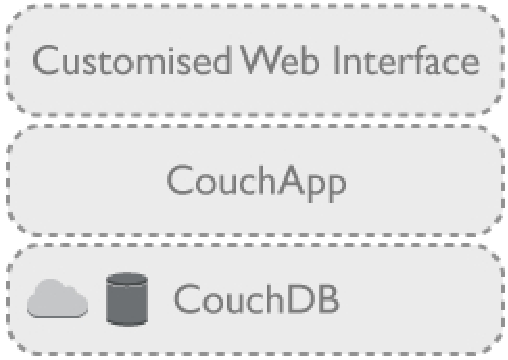
\includegraphics[width=0.5\textwidth]{images/data-centre-app-stack.pdf}
    \caption{Social Network IoT Sensing Application Layer Stack}
    \label{fig:data-centre-app-stack}
  \end{center}
\end{figure}

CouchDB acts as an HTTP server, serving HTML directly to a browser, while manages heterogeneous data and horizontal scaling; CouchDB, moreover, provides live notifications and handles over the notifications to upper layers. External data, such as collected by IoT devices, connect to CouchDB via a gateway. The collection of the data and the purpose of the gateway have been discussed in \cite{francesco2012storage}. 

CouchApp inherited these features from CouchDB. Furthermore, CouchApp is extensible. Thus, we have a third layer to extend the functionality and customise the usability. For instance, we used BackboneJS, Model-View (MV) Javascript library, to structure our application. Third party APIs, additionally, can be integrated into the third layer and thus enable, e.g. social network or geography functions. End users interact with the system via the third layer. 

The architecture of the sample application is shown in Figure \ref{fig:data-centre-architecture}.

\begin{figure}[ht]
  \begin{center}
    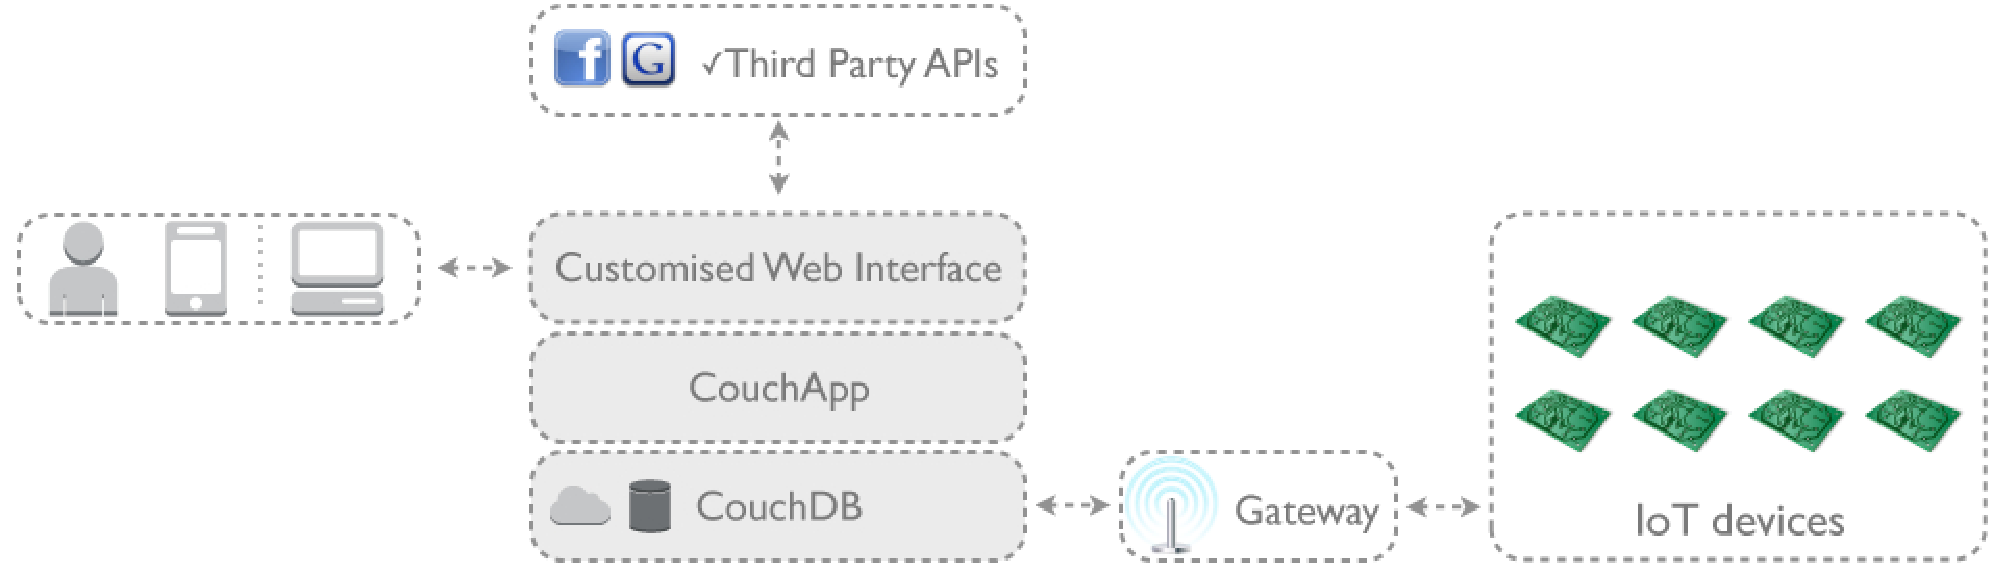
\includegraphics[width=1\textwidth]{images/data-centre-architecture.pdf}
    \caption{Social Network IoT Sensing Application Architecture \cite{francesco2012storage}}
    \label{fig:data-centre-architecture}
  \end{center}
\end{figure}

\subsection{Retrieving Data}
The architecture, which end users directly interacting with, is based on a HTTP web server, CouchDB. Thus, all connections are HTTP based. In order to keep notification alive, the browser has to maintain HTTP connections, negotiate with the web server, update HTTP connections and keep HTTP connection alive. 


 